\documentclass[17pt]{beamer} %Makes presentation
%\documentclass[handout, 17pt]{beamer} %Makes Handouts
\usetheme{Singapore} %Gray with fade at top
\useoutertheme[subsection=false]{miniframes} %Supppress subsection in header
\useinnertheme{rectangles} %Itemize/Enumerate boxes
\usecolortheme{seagull} %Color theme
\usecolortheme{rose} %Inner color theme

\definecolor{light-gray}{gray}{0.75}
\definecolor{dark-gray}{gray}{0.55}
\setbeamercolor{item}{fg=light-gray}
\setbeamercolor{enumerate item}{fg=dark-gray}

\setbeamertemplate{navigation symbols}{}
%\setbeamertemplate{mini frames}[default]
%\setbeamercovered{dynamics}
\setbeamerfont*{title}{size=\Large,series=\bfseries}
\setbeamerfont{footnote}{size=\tiny}

%\setbeameroption{notes on second screen} %Dual-Screen Notes
%\setbeameroption{show only notes} %Notes Output

\setbeamertemplate{frametitle}{\vspace{.5em}\bfseries\insertframetitle}
\newcommand{\heading}[1]{\noindent \textbf{#1}\\ \vspace{1em}}

\usepackage{bbding,color,multirow,times,ccaption,tabularx,graphicx,verbatim,booktabs}
\usepackage{colortbl} %Table overlays
\usepackage[english]{babel}
%\usepackage[latin1]{inputenc}
%\usepackage[T1]{fontenc}
\usepackage{lmodern}

%\author[]{Thomas J. Leeper}
\institute[]{
  \inst{}%
  Department of Government\\London School of Economics and Political Science
}

\usepackage{tikz}
\usetikzlibrary{shapes,arrows}

\title{\large{Causality:\\Explanation versus Prediction}}

% Political science is generally concerned with questions of causality. To do that we need to learn to think counterfactually. How do we know that something causes something else? How do we separate ``correlation'' from ``causation''?

\date[]{}

\begin{document}

\frame{\titlepage}

\frame{\tableofcontents}


% talk about "identification"

% constants can't be used to understand causality because we don't get to see counterfactuals



\section[MT]{Brief Review of MT Material}
\frame{\tableofcontents[currentsection]}

\frame{\huge\vskip20pt\textbf{What did we learn about during MT?}}

% research questions; what makes questions interesting
% concept definition
% operationalization
% what does it mean to describe?
% texts as data
% interviews as data
% what are ``cases''?
% representativeness
% ethics


\frame{
\frametitle{New territory\dots}

By the end of today you should be able to:

\begin{itemize}
\item Identify what makes for a causal relationship
\item Distinguish causation from correlation/association
\item Begin to analyse research problems using counterfactual thinking
\end{itemize}

}

\frame{
\frametitle{The broad story arc for LT}

\begin{itemize}\itemsep1em
\item<1-> Causal inference!
	\begin{itemize}
	\item Generating causal theories and expectations
	\item Making comparisons
	\item Statistical methods useful for causal inference
	\item (Quasi-)Experimentation
	\end{itemize}
\item<2-> Developing your research proposals
	\begin{itemize}
	\item One-on-ones w/ Thomas
	\item Literature review (Reading Week)
	\end{itemize}
\end{itemize}

}


% Today: focusing on what it means for something to be a ``cause''

% Goal is to develop ways of thinking about how to distinguish causation from association/correlation

% where do we look for counterfactuals? backward or forward in time? across similar cases?


\section{Causality}
\frame{\tableofcontents[currentsection]}

\frame{

\frametitle{Pre-Post Change Heuristic}

\begin{itemize}\itemsep1em
\item Our intuition about causation relies too heavily on simple comparisons of \textit{pre-post change} in outcomes before and after something happens

	\begin{itemize}
	\item No change: no causation
	\item Increase in outcome: positive effect
	\item Decrease in outcome: negative effect
	\end{itemize}

\item Several reasons why this is inadequate!
\end{itemize}

}

\frame{

\frametitle{Flaws in causal inference from pre-post comparisons}

\begin{enumerate}
\item Maturation or trends
\item Regression to the mean
\item Selection
\item Simultaneous historical changes
\item Instrumentation changes
\item Monitoring changes behaviour
\end{enumerate}

}


% Causal graphs

\frame{

\frametitle{{\large Directed Acyclic Graphs}}

\small

\begin{itemize}\itemsep0.5em
\item Causal graphs (DAGs) provide a visual representation of (possible) causal relationships
\item<2-> Causality flows between variables, which are represented as ``nodes''
	\begin{itemize}
	\item Variables are causally linked by arrows
	\item Causality only flows \textit{forward} in time
	\end{itemize}
\item<3-> Nodes opening a ``backdoor path'' from $X \rightarrow Y$ are confounds
	\begin{itemize}
	\item ``Selection bias'' or ``Confounding''
	\end{itemize}
\end{itemize}

}


\begin{frame}[label=smoking-graph]
\begin{center}
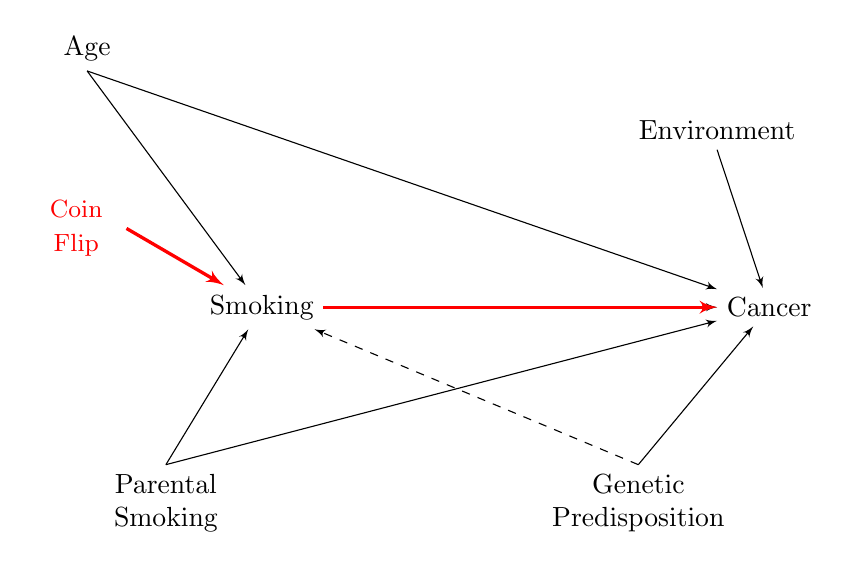
\begin{tikzpicture}[>=latex',circ/.style={draw, shape=circle, node distance=5cm, line width=1.5pt}]
    \draw (0,0) node[left] (X) {Smoking};
    \draw[->] (X) -- (5,0) node[right] (Y) {Cancer};
    \draw<2->[->] (-3,3) node[above] (Z) {Age} -- (Y);
    \draw<2->[->] (5,2) node[above] (A) {Environment} -- (Y);
    \draw<2->[->] (4,-2) node[below, text width=3cm, align=center] (E) {Genetic\\Predisposition} -- (Y);
    \draw<2->[->] (-2, -2) node[below, text width=2.5cm, align=center] (W) {Parental\\Smoking} -- (Y);
    \draw<3->[->] (Z.south) -- (X);
    \draw<3->[->] (W.north) -- (X);
    \draw<4->[->, dashed] (E.north) -- (X);
    %\draw<4->[<->, dashed] (W.west) -- (X.west);

    \draw<5->[->, very thick, color=red] (-2.5,1) node[left, color=red, text width=1cm, align=center] (Tr) {\small Coin\\ Flip} -- (X);
    \draw<5->[->, very thick, color=red] (X) -- (Y);
\end{tikzpicture}
\end{center}
\end{frame}


\frame<1-2>[label=causality]{

\frametitle{{\large The 3 or 4 or 5 principles}}

\begin{enumerate}\itemsep1em
\item<2-> Correlation
\item<3-> Nonconfounding
\item<4-> Direction (``temporal precedence'')
\item<5-> Mechanism
\item<6-> (Appropriate level of analysis)
\end{enumerate}
}

\againframe<2>{smoking-graph}

\againframe<2-3>{causality}

\againframe<2-4>{smoking-graph}

\againframe<3-4>{causality}

\againframe<4>{smoking-graph}

\againframe<4->{causality}

\frame{
	\centering
	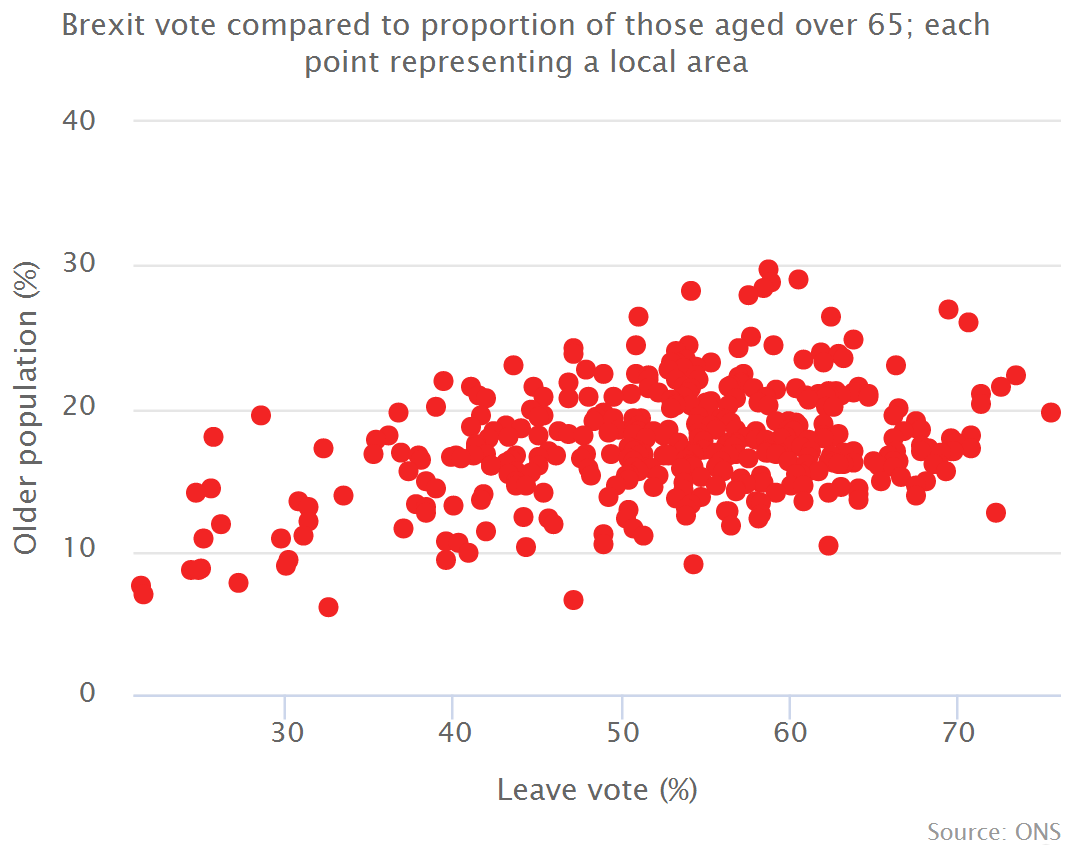
\includegraphics[width=.9\textwidth]{images/brexit-vote-by-age.png}
	
	{\tiny Source: \textit{The Telegraph}. 27 June 2016. \url{http://www.telegraph.co.uk/news/2016/06/24/eu-referendum-how-the-results-compare-to-the-uks-educated-old-an/}\par }
}


\frame{\huge\vskip20pt\textbf{Questions?}}



\section[Counterfactuals]{Fundamental Problem of Causal Inference}
\frame{\tableofcontents[currentsection]}

\frame{

\frametitle{Causal Inference}

\centering

Causal inference (typically) involves gathering data in a systematic fashion in order to assess the size and form of correlation between nodes $X$ and $Y$ in such a way that there are no backdoor paths between $X$ and $Y$ by \textit{controlling for} (i.e., \textit{conditioning on}, \textit{holding constant}) any confounding variables, $\mathbf{Z}$.

}


\frame{

\large\centering

In essence, this means finding or creating \textit{counterfactuals}.

}

\frame[label=counterfactuals]{
\frametitle{Counterfactual Thinking}

\begin{itemize}\itemsep1.5em
\item Causal inference involves inferring \textit{what would have happened} in a counterfactual reality \textit{where the potential cause took on a different value}
\item \textit{Counterfactual}: relating to what has not happened or is not the case
\end{itemize}

}

% Has anyone read or seen *A Christmas Carol*?

\frame{
\frametitle{``A Christmas Carol''}

\small 
\begin{itemize}
\item 1843 novel by Charles Dickens
\item Ebenezer Scrooge is shown his own future by the ``Ghost of Christmas Yet to Come''
\item Has the choice to either:
	\begin{enumerate}\footnotesize
	\item stay on current path (one counterfactual), or 
	\item change his ways (take a different counterfactual)
	\end{enumerate}
\end{itemize}
}


\frame{
\frametitle{{\large Dickensian Causal Inference}}

\begin{itemize}\itemsep1em
\item \textit{Causal effect}: The difference between two ``potential outcomes''
	\begin{itemize}
	\item The outcome that occurs if $X = x_1$
	\item The outcome that occurs if $X = x_2$
	\end{itemize}
\item The causal effect of Scrooge's lifestyle is seen in the \textit{difference(s)} between two potential futures
\end{itemize}

}

\frame{

\frametitle{Other Counterfactuals\\ in TV \& Film}


\begin{itemize}
\item \textit{Groundhog Day}
\item \textit{Run Lola Run}
\item \textit{Minority Report}
\item \textit{Source Code}
\item \textit{X-Men: Days of Future Past}
\end{itemize}

}


\frame{
\frametitle{Fundamental problem of causal inference!}

\large\centering We can only observe any given unit in one reality! So any counterfactual for a given unit is unobservable!!!

\vspace{1em}

\only<2->{OH NO!}

}

\frame{
\frametitle{Two solutions!}

\begin{enumerate}\itemsep1em
\item ``Scientific'' Solution\footnote{From Holland}
	\begin{itemize}
	\item (Assume) units are all identical
	\item Each can provide a perfect counterfactual
	\item Common in, e.g., agriculture, biology
	\end{itemize}
\item<2-> ``Statistical'' Solution
	\begin{itemize}
	\item Units are not identical
	\item Random exposure to a potential cause
	\item Effects measured on average across units
	\item Known as the ``Experimental ideal''
	\end{itemize}
\end{enumerate}

}


\frame<1>[label=mill]{

\frametitle{Mill's methods\footnote{Discussed in Holland}}

\begin{itemize}
\item Agreement
\item \textbf<2>{Difference}
\item Agreement and Difference
\item Residue
\item Concomitant variations
\end{itemize}
}

\frame{
\frametitle{{\normalsize Mill's Method of Difference}}

``If an instance in which the phenomenon under investigation occurs, and an instance in which it does not occur, have every circumstance save one in common, that one occurring only in the former; the circumstance in which alone the two instances differ, is the effect, or cause, or an necessary part of the cause, of the phenomenon.''
}


\frame{

\frametitle{{\large ``Rerum cognoscere causas''}}

\begin{itemize}
\item<1-> Causal inference is meant to help ``explain'' the social world
	\begin{itemize}
	\item<2-> Other notions of \textit{explain}
		\begin{itemize}
		\item Concept generation and labelling
		\item Descriptive typologies
		\end{itemize}
	\item<3-> Explanation may or may not involve mechanistic claims (see LT Week 5)
	\end{itemize}
\item<4-> Causation is deterministic at the unit level!
\item<5-> Counterfactual approaches to causal inference are ``forward'' in nature
\end{itemize}

}

\frame{
\centering
Prediction is not causation.\\ Causation is not prediction.

\vspace{2em}

\only<2->{Why are these distinct?}

}




\section{Randomized Experiments}
\frame{\tableofcontents[currentsection]}





% Individual-level effects versus ATEs


\frame{
	\frametitle{The Experimental Ideal}
	\small
	A randomized experiment, or randomized control trial is:
 		\begin{quote}\small
 			The observation of units after, and possibly before, a randomly assigned intervention in a controlled setting, which tests one or more precise causal expectations
 		\end{quote}
 	This is Holland's ``statistical solution'' to the fundamental problem of causal inference
}

\frame{
	\frametitle{Random Assignment}

\small
\begin{itemize}\itemsep0.5em
\item A physical process of randomization
	\begin{itemize}\small
	\item Breaks the ``selection process''
	\item Units only take value of $X = x$ because of assignment
	\end{itemize}
\item<2-> This means:
	\begin{itemize}\small
	\item Treatment groups, on average, provide in sight into counterfactual ``potential'' outcomes
	\item Randomization means potential outcomes are balanced between groups, so no confounding
	\end{itemize}
\end{itemize}

}


\againframe<5->{smoking-graph}


% design-based experimental inference
\frame{
	\frametitle{Experimental Inference I}
	\small
	\begin{itemize}\itemsep0.5em
    	\item<1-> Causal inference is a comparison of two \textit{potential outcomes}
    	\item<2-> A potential outcome is the value of the outcome ($Y$) for a given unit (i) after receiving a particular version of the treatment ($X$)
    	\item<3-> Each unit has multiple \textit{potential} outcomes ($y_{0i}$, $y_{1i}$), but we only observe one of them
    	\item<4-> A \textit{causal effect} is the difference between these (e.g., $y_{x=1} - y_{x=0}$), all else constant
	\end{itemize}
}

\frame{
	\frametitle{Experimental Inference II}
	\small
	\begin{itemize}\itemsep0.5em
    	\item<1-> We cannot see individual-level causal effects
			\begin{itemize}
			\item<1-> We want to know: $TE_i = y_{1i} - y_{0i}$
			\end{itemize}
    	\item<2-> We can see \textit{average causal effects}
    		\begin{itemize}
        		\item<2-> Ex.: Average difference in cancer between those who do and do not smoke
        		\item<2-> $ATE_{naive} = E[y_{1i} | x_{i} = 1] - E[y_{0i} | x_{i} = 0]$
    		\end{itemize}
    	\item<3-> Is this what we want to know?
    		\begin{itemize}
    		\item<4-> Yes, if $X$ randomized
    		\item<5-> Yes, if all confounds controlled
    		\end{itemize}
	\end{itemize}
}


\frame{}




\frame{

\frametitle{Preview of next week}

\begin{itemize}\itemsep1em
\item What is a ``scientific literature''?
\item How do we accumulate scientific evidence?
\end{itemize}

}


\appendix
\frame{}

\frame{\frametitle{Mill's Methods}}

\frame{
\frametitle{Agreement}

If two or more instances of the phenomenon under investigation have only one circumstance in common, the circumstance in which alone all the instances agree, is the cause (or effect) of the given phenomenon.
}

\frame{
\frametitle{Difference}

If an instance in which the phenomenon under investigation occurs, and an instance in which it does not occur, have every circumstance save one in common, that one occurring only in the former; the circumstance in which alone the two instances differ, is the effect, or cause, or an necessary part of the cause, of the phenomenon.
}

\frame{
\frametitle{Agreement and Difference}

If two or more instances in which the phenomenon occurs have only one circumstance in common, while two or more instances in which it does not occur have nothing in common save the absence of that circumstance; the circumstance in which alone the two sets of instances differ, is the effect, or cause, or a necessary part of the cause, of the phenomenon.
}

\frame{
\frametitle{Residue}

Subduct from any phenomenon such part as is known by previous inductions to be the effect of certain antecedents, and the residue of the phenomenon is the effect of the remaining antecedents.
}

\frame{
\frametitle{Concomitant variations}

Whatever phenomenon varies in any manner whenever another phenomenon varies in some particular manner, is either a cause or an effect of that phenomenon, or is connected with it through some fact of causation.
}


\end{document}
